\documentclass[a4paper]{article}
\setlength{\topmargin}{-1.0in}
\setlength{\oddsidemargin}{-0.2in}
\setlength{\evensidemargin}{0in}
\setlength{\textheight}{10.5in}
\setlength{\textwidth}{6.5in}
\usepackage{enumitem}
\usepackage{amsmath}
\usepackage{hyperref}
\usepackage{amssymb}
\usepackage[dvipsnames] {xcolor}
\usepackage{mathpartir}
\usepackage{graphicx}
\usepackage{tikz}
\usetikzlibrary{positioning,arrows.meta}

\hbadness=10000

\hypersetup{
    colorlinks=true,
    linkcolor=blue,
    filecolor=magenta,      
    urlcolor=cyan,
    pdftitle={Assignment 2},
    pdfpagemode=FullScreen,
    }
\def\endproofmark{$\Box$}
\newenvironment{proof}{\par{\bf Proof}:}{\endproofmark\smallskip}
\begin{document}
\begin{center}
{\large \bf \color{red}  Department of Computer Science} \\
{\large \bf \color{red}  Ashoka University} \\

\vspace{0.1in}

{\large \bf \color{blue}  Introdution to Quantitative Finance}

\vspace{0.05in}

    { \bf \color{YellowOrange} Assignment 3}
\end{center}
\medskip

\hfill {\textbf{Name: Rushil Gupta} }

\bigskip
\hrule


% Begin your assignment here %

\section*{Question 1}
\begin{enumerate}[label=(\alph*)]
    \item The payoff diagram for the portfolio is shown below: \\
    \begin{align*}
        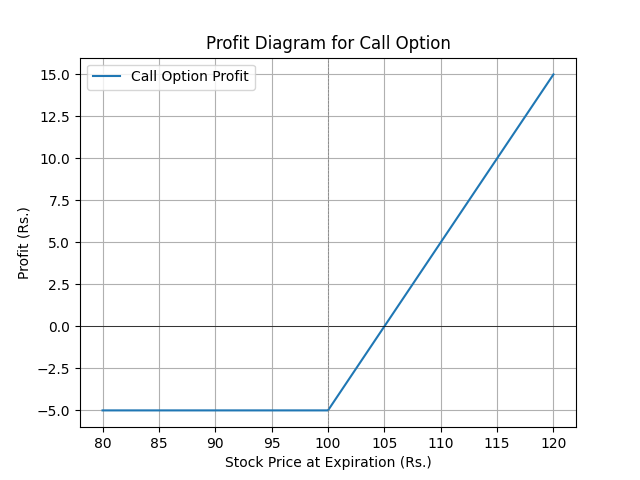
\includegraphics[width=0.7\textwidth]{q1a.png}
    \end{align*}

    At price $S_T = 102$, we would not make a profit, since our payoff of the option is 2, and the premium of the option is 5. This means that we would lose 3 Rs. But, since we already have the option and have already paid the premium, we would exercise the option to reduce our loss from 5 Rs. to 3 Rs.

    \vspace{5mm}
    \item The profit diagram for the portfolio is shown below: \\
    \begin{align*}
        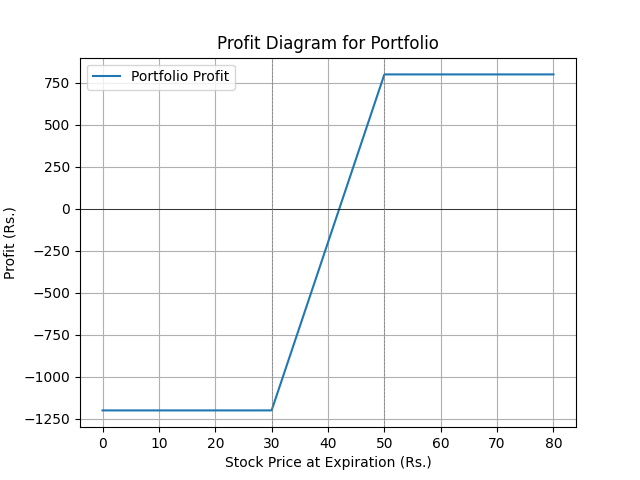
\includegraphics[width=0.7\textwidth]{q1b.png}
    \end{align*}
\end{enumerate}

\newpage
\section*{Question 2}


\begin{enumerate}[label=(\alph*)]
    \item We know that $C + Ke^{-rT} = P + S_0$. We already know that $C = 1$, $K = 20$, $r = 0.04$, and $S_0 = 19$. \\
 
    Since we are assuming continuous compounding, we have $e^{-rT} = e^{-0.04 \times 0.25} = e^{-0.01} \approx 0.9900$. \\

    This gives us:
    \[ 1 + 20 \times 0.9900 = P + 19 \]
    \[ \implies P = 1.8 \]

    So, the price of the put option is Rs. 1.80.

    \vspace{4mm}
    \item The payoff diagram for the portfolio is shown below: \\
    \begin{align*}
        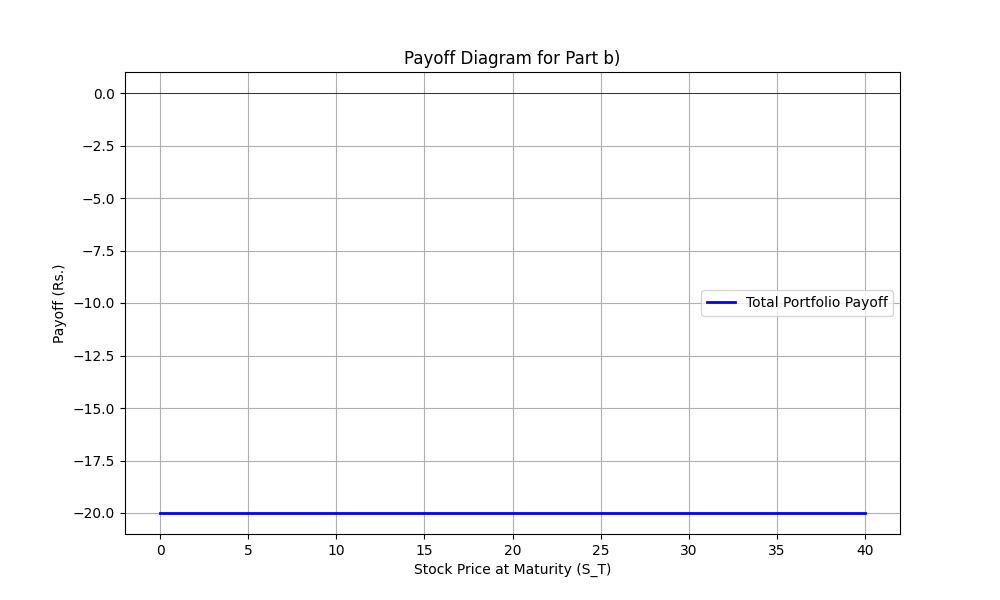
\includegraphics[width=0.7\textwidth]{q2b.png}
    \end{align*}

    \item The payoff diagram for the portfolio is shown below: \\
    \begin{align*}
        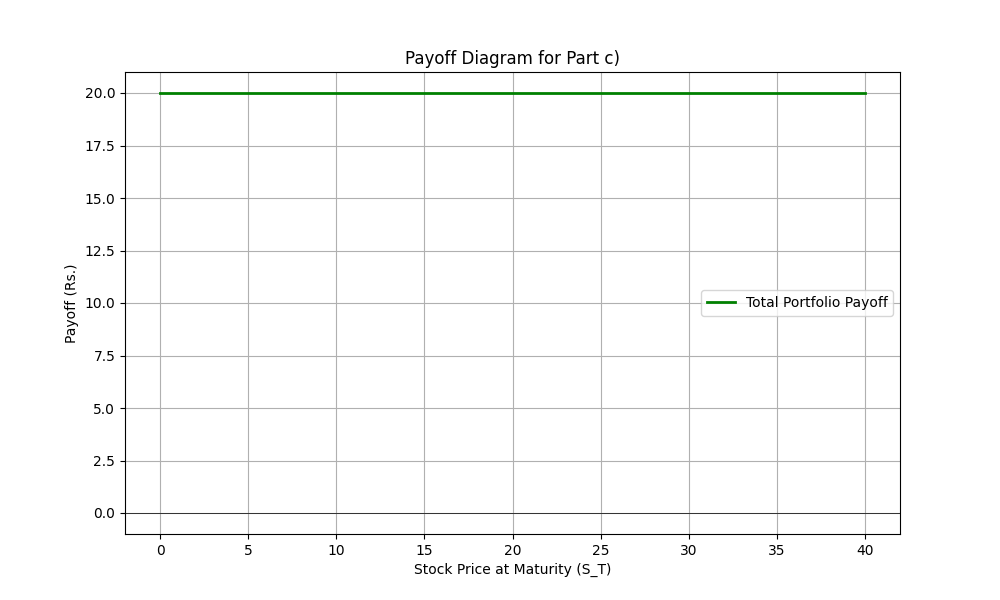
\includegraphics[width=0.7\textwidth]{q2c.png}
    \end{align*}

    \item In part b, we see that the payoff is constant at Rs. -20 for all stock prices. Looking at the cost of the portfolio, we see that the cost is $\text{Rs.} -19.80 = -19 - 1.80 + 1$. This means, the return made here is $0.2/19.80 = 1.01\%$, which is the same as the risk free rate. \\

    In part c, we see that the payoff is constant at Rs. 20 for all stock prices. Looking at the cost of the portfolio, we see that the cost is $\text{Rs.} 19.80 = 19 + 1.80 - 1$. This means, the return made here is $0.2/19.80 = 1.01\%$, which is the same as the risk free rate. \\

    So, we see that in both cases, the return made is the same as the risk free rate, which shows us how options can be used to mimic risk free assets.
\end{enumerate}


\newpage
\section*{Question 3}

\begin{enumerate}[label=(\alph*)]
    \item We start by calculating the price of the put option. We will use the following formula:
    
    \[ P = Ke^{-rT} - S_0 + C + PV(D) \]

    Where, $PV(D)$ is the present value of the dividends. Hence, we can calcuate $PV(D)$ as follows:

    \[ PV(D) = 0.5e^{-0.1 \times 2/12} + 0.5e^{-0.1 \times 5/12} \]
    \[ = 0.4918 + 0.4796 \]
    \[ = 0.9714 \]

    Now, we can calculate the price of the put option as follows:

    \[ P = 30e^{-0.1 \times 0.5} - 29 + 2 + 0.9714 \]
    \[ = 28.537 - 29 + 2 + 0.9714 \]
    \[ = 2.5084 \]

    So, the price of the put option is Rs. 2.5084. To exploit arbitrage, we see that the put is currently overpriced. Hence, we can make a portfolio with the following instruments:
    \begin{itemize}
        \item Sell the put option for Rs. 3
        \item Buy the call option for Rs. 2
        \item Short sell the stock for Rs. 29
        \item Invest the present value of the strike price ($= 28.537$) in the bank for 6 months at 10\% per annum.
        \item Invest the present value of the dividend ($= 0.9714$) in the bank for 6 months at 10\% per annum.
    \end{itemize}

    The cost of the portfolio is $+3 - 2 + 29 - 28.537 - 0.9714 = 0.4916$. \\

    Now, we need to calculate the payoff of the portfolio at maturity. If the stock price at maturity is $S_T$, then:

    Case 1: $S_T \leq 30$
    \begin{itemize}
        \item The call option is not exercised, since we have a 0 payoff.
        \item To close the short position in the stock, we exercise the put option and buy the stock at price $S_T$.
        \item The cost of exercising the put option is Rs. $30$, which is what our initial investment of $28.537$ grew to.
        \item We also use the $0.9714$ that we invested in the bank to pay the dividents the stock was expected to give.
    \end{itemize}

    So, our final cash outflow is 0. This means, we got Rs. 0.4916 riskless profit. Similarly, if $S_T \geq 30$, we can calculate the final cash inflow to be Rs. 0.4916.


    \vspace{5mm}
    \item We need to show that $c - S_0 + Ke^{-rLT} \geq p \geq c - S_0 + Ke^{-rBT}$.

    \begin{proof}
        \\
        \textbf{Case 1}: Suppose $p \geq c - S_0 + Ke^{-r_l T}$

        Then, we can sell the put option, buy the call option, and invest in the bank at rate $r_l$. This way, our portfolio will have a positive cost ($C_0 > 0$), and zero payoff at maturity. Hence, we can exploit this arbitrage opportunity. So, $p \geq c - S_0 + Ke^{-r_l T}$. \\

        \textbf{Case 2}: Suppose $p \leq c - S_0 + Ke^{-r_b T}$

        Then, we can buy the put option, sell the call option, and invest in the bank at rate $r_b$. This way, our portfolio will have a positive cost ($C_0 > 0$), and zero payoff at maturity. Hence, we can exploit this arbitrage opportunity. So, $p \leq c - S_0 + Ke^{-r_b T}$.

        Hence, we have shown that $p \geq c - S_0 + Ke^{-r_l T}$ and $p \leq c - S_0 + Ke^{-r_b T}$, which gives us the required inequality.
    \end{proof}

    \newpage
    \item Using the formula from part b, we can calculate the bounds on the price of the put option as follows:
    
    \[ PV(D) = 0.9714 \]

    So: 
    \[S_0' = S_0 - PV(D) = 29 - 0.9714 = 28.0286 \]

    Then, 
    \[ Ke^{-r_lT} = 30e^{-0.1 \times 0.5} = 28.537 \]
    \[ Ke^{-r_bT} = 30e^{-0.1 \times 0.5} = 28.253 \]

    Using the inequality from part b, we get:
    \[ c - S_0' + Ke^{-r_lT} \geq p \geq c - S_0' + Ke^{-r_bT} \]
    \[ \implies 2 - 28.0286 + 28.537 \geq p \geq 2 - 28.0286 + 28.253 \]
    \[ \implies 2.5084 \geq p \geq 2.2244 \]
\end{enumerate}


\vspace{10mm}
\section*{Question 4}
% Three put options on a stock have the same expiration date and strike prices of Rs. 55, Rs. 60, and Rs. 65. The market prices are Rs. 3, Rs. 5, and Rs. 8, respectively. Explain how a butterfly spread can be created. Construct a table showing the profit from the strategy. For what range of stock prices would the butterfly spread lead to a loss?

The butterfly spread can be made with the following portfolio:
\begin{itemize}
    \item Buy one put option with strike price Rs. 55 for Rs. 3
    \item Sell two put options with strike price Rs. 60 for Rs. 5 each
    \item Buy one put option with strike price Rs. 65 for Rs. 8
\end{itemize}

The initial cost of the portfolio is $- 3 + 2 \times 5 - 8 = -1$. So, spend Rs. 1 to make the portfolio.

The profit from the strategy is shown in the table below:
\begin{align*}
    \begin{tabular}{|c|c|c|c|c|c|}
        \hline
        Stock Price & K=55 & K=60 & K=65 & Option Payoff & Net Payoff \\
        \hline
        $S_T \leq 55$ & $55 - S_T$ & $2 \times (S_T - 60)$ & $65 - S_T$ & $0$ & $-1$\\
        \hline
        $55 < S_T < 60$ & $0$ & $2 \times (S_T - 60)$ & $65 - S_T$ & $S_T - 55$ & $S_T - 56$ \\
        \hline
        $S_T = 60$ & $0$ & $0$ & $5$ & $5$ & $4$ \\
        \hline
        $60 < S_T < 65$ & $0$ & $0$ & $65 - S_T$ & $65 - S_T$ & $64 - S_T$ \\
        \hline
        $S_T \geq 65$ & $0$ & $0$ & $0$ & $0$ & $-1$ \\
        \hline
    \end{tabular}
\end{align*}

So, we see that we make losses whenever $S_T < 56$ or $S_T > 64$. The maximum loss is Rs. 1, while the maximum profit is Rs. 4, at $S_T = 60$.


\vspace{10mm}
\section*{Question 5}
% A stock currently trades at Rs. 50, and we are looking to determine the price of a European call option on this stock using a two-period binomial model. The following information is provided:

In this section, we will show the calcuations for one of the strike prices. The rest of the calculations will be done in the same way, and then the plot of the option price against the strike price will be shown. \\

Firstly, we have $r = 5\%$, and by assuming continuous compounding, we have $u = e^r = e^0.05 \approx 1.0513$. We will calculate the option price for a strike price of Rs. 50. \\

Now, at $t = 2$, we have:
\[ S_2(HH) = 1.2^2 \times 50 = 72 \]
\[ S_2(HT) = S_2(TH) = 1.2 \times 0.8 \times 50 = 48 \]
\[ S_2(TT) = 0.8^2 \times 50 = 32 \]

Then, the payoffs at $t = 2$ are:
\[ X_2(HH) = \max(72 - 50, 0) = 22 \]
\[ X_2(HT) = P_2(TH) = \max(48 - 50, 0) = 0 \]
\[ X_2(TT) = \max(32 - 50, 0) = 0 \]

Now, we can find $X_1$ by using the formula for $X_n$ as:

\[ X_n(x_1, x_2, ..., x_n) = e^{-r} \left( \tilde{p} X_{n+1}(x_1, x_2, ..., x_n, H) + \tilde{q} X_{n+1}(x_1, x_2, ..., x_n, T) \right) \] \\

First, we find $\tilde{p}$ and $\tilde{q}$:

\[ \tilde{p} = \frac{e^{r} - d}{u - d} = \frac{1.0513 - 0.8}{1.2 - 0.8} = 0.628 \]
\[ \tilde{q} = 1 - \tilde{p} = 0.372 \]

Then, we can find $X_1$ as follows:

\[ X_1(H) = e^{-0.05} \left( 0.628 \times 22 + 0.372 \times 0 \right) = 13.14 \]
\[ X_1(T) = e^{-0.05} \left( 0.628 \times 0 + 0.372 \times 0 \right) = 0 \] \\

Then, the price of the call option is $X_0$:

\[ X_0 = e^{-0.05} \left( 0.628 \times 13.14 + 0.372 \times 0 \right) = 7.85 \]


Similarly, we can calculate the price of the call option for other strike prices. The plot of the option price against the strike price is shown below:

\begin{align*}
    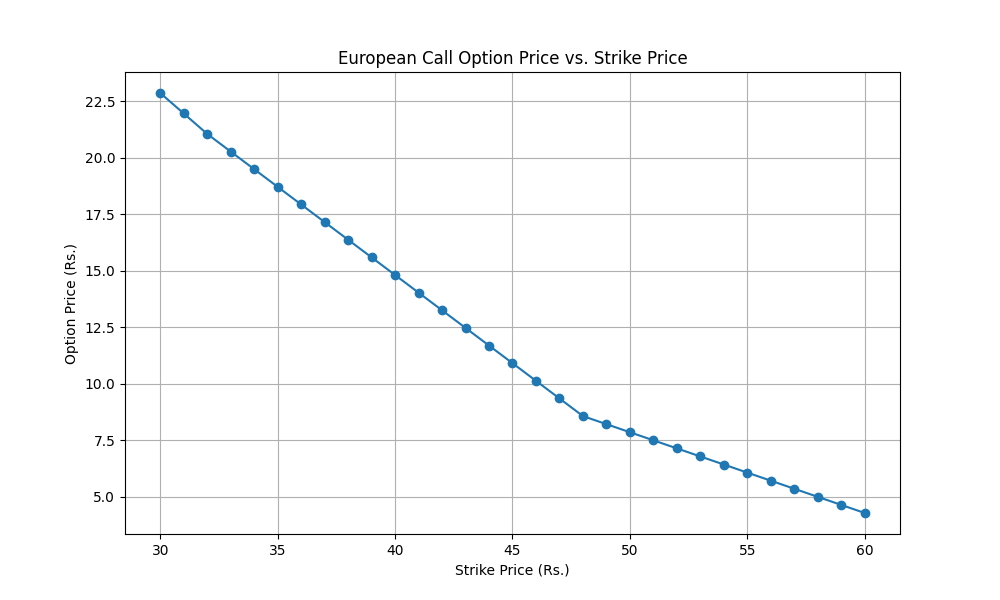
\includegraphics[width=0.8\textwidth]{q5.png}
\end{align*}

\newpage
\section*{Question 6}
% A stock price is currently Rs. 30. During each 2-month period for the next 4 months, it will increase by 8% or reduce by 10%. The risk-free interest rate is 5% per annum (assume continuous compounding).

\begin{enumerate}[label=(\alph*)]
    % Use a two-step tree to calculate the value of a European-style derivative that pays off max(30 − ST , 0)^2, where ST is the stock price after 4 months.

    \item At $t = 2$, we have:
    \[ S_2(HH) = 1.08^2 \times 30 = 34.992 \]
    \[ S_2(HT) = S_2(TH) = 1.08 \times 0.9 \times 30 = 29.16 \]
    \[ S_2(TT) = 0.9^2 \times 30 = 24.3 \]

    We can find the payoffs at $t = 2$ as follows:
    \[ X_2(HH) = \max(30 - 34.992, 0)^2 = 0 \]
    \[ X_2(HT) = X_2(TH) = \max(30 - 29.16, 0)^2 = 0.7056 \]
    \[ X_2(TT) = \max(30 - 24.3, 0)^2 = 32.49 \]

    Now, using the same method as in question 5, we can find the price of the derivative at $t = 1$ as follows:

    \[ \tilde{p} = \frac{e^{r \times 2 / 12} - d}{u - d} = \frac{1.0084 - 0.9}{1.08 - 0.9} = 0.602 \]
    \[ \tilde{q} = 1 - \tilde{p} = 0.398 \]

    \[ X_1(H) = e^{-0.05 \times 2 / 12} \left( 0.602 \times 0 + 0.398 \times 0.7056 \right) = 0.2785 \]
    \[ X_1(T) = e^{-0.05 \times 2 / 12} \left( 0.602 \times 0.7056 + 0.398 \times 32.49 \right) = 13.245 \]

    Finally, the price of the derivative at $t = 0$ is:
    \[ X_0 = e^{-0.05 \times 2 / 12} \left( 0.602 \times 0.2785 + 0.398 \times 13.245 \right) = 5.394 \]


    \vspace{5mm}
    % If the derivative is American-style, should it be exercised early?
    \item If the derivative is American-style, we have the option to exercise the derivative at $t = 1$ or $t = 2$. For this, we will calculate $V_1$ for both $H$ and $T$ at $t = 1$, and compare it with the payoff at $t = 1$ for both $H$ and $T$.

    \[ V_1(H) = \max(30 - 1.08 \times 30, 0)^2 = 0.107 \]
    \[ V_1(T) = \max(30 - 0.9 \times 30, 0)^2 = 9 \]

    In this case, we would never exercise the option early since the payoff at $t = 0, 1$ is less than the expected payoff at $t = 2$. However, in a more realistic scenario, we would exercise the option early if the stock falls sharply, since the payoff increases quadratically as the stock price falls.
\end{enumerate}


\newpage
\section*{Question 7}

% Consider a one-period trinomial tree model as shown in the figure below. The stock price at time t = 0, denoted by S0, is Rs. 10. After one time period (one year), the stock price can move to one of three possible values: Rs. 12 (i.e. Su), Rs. 10 (i.e. Sm), or Rs. 8 (i.e. Sd). Consider the risk-free rate as 10% per annum (assume continuous compounding). Find all the possible prices of a call option with a strike price of Rs. 9 such that there is no arbitrage opportunity.

% The tree shown is

% S_0
% -> S_u
% -> S_m
% -> S_d

We first start by looking at the payoffs of the call option at each node.

\[ V_1(u) = \max(12 - 9, 0) = 3 \]
\[ V_1(m) = \max(10 - 9, 0) = 1 \]
\[ V_1(d) = \max(8 - 9, 0) = 0 \]

Also, since we have a time period of 1 year and $r_c = 0.10$, with continuous compounding, we have $r = e^{r_c} = e^{0.10} \approx 1.1052$. \\

Now, the goal is to create a portfolio that will have the same payoff as the call option at $t = 1$, and will have no arbitrage opportunity. However, in this case, we have 3 equations and 2 unknowns, so we know that we cannot solve for this. Therefore, we will use inequalities to find the range of possible prices. \\

Define $x$ to be the amount of money invested in the stock, and $y$ to be the amount of money invested in the bank. Then:

\begin{align}
    x \times 12 + y \times 1.1052 &\leq 3 \\
    x \times 10 + y \times 1.1052 &\leq 1 \\
    x \times 8 + y \times 1.1052 &\leq 0
\end{align}

We are using the inequalities because we know we cannot have a portfolio with a higher payoff than the call option due to the no arbitrage principle. However, we can have a portfolio with a lower payoff than the call option. \\

With these conditions, we want to minimize $P$, the price of the call option. $P$ is given by:

\[ P = x \times 10 + y \]

Now, to solve the constraints, we use a python based PuLP model. It gives:

\[ 1.86 \leq P \leq 2.07 \]

This means that if $P$ is outside this range, we can exploit arbitrage opportunities.





\end{document}